\secput*{Preprocessing}

This section describes how a range coalescing data structure is built cache-obliviously
from a set of $k$ $n$-length sorted lists $L_1 \ldots L_k$ and bounds
the number of memory transfers incurred by the process.  We do this in four steps.
First, we give a suboptimal deterministic strategy for finding the splitters 
--- the values that partition the query space such that each partition has $O(k)$ 
elements from the constituent lists in $\{ L_1 \ldots L_k \}$.  Second, we 
demonstrate that the elements from each list can be assembled in the bin corresponding
to each splitter using $O(N / B)$ memory transfers, for $N=nk$.  
Finally, we give two randomized algorithm for finding the splitters when 
$k < \lg^2 n$ and $k \geq \lg^ n$, 
respectively, each of which incurs $O(N/B)$ memory transfers.  

\subsection*{Preprocessing suboptimally}

In this section, we show how to find an $n$-length sorted splitter array $S$, such that $O(k)$
elements from $\mathcal{L} = \cup_{i=1}^{k}L_i$ fall in each range 
$[S_j,S_{j+1})$ $\forall j$.  If we assume that all elements in $\mathcal{L}$ are 
unique, we can merely merge all the elements and take every $k$th element in the
merged list as the splitters.\footnote{We can extend the value of each element with the
list number in order to make them unique, since the elements from any particular
list $L_i$ are unique.  Note that if each list contained a value $l$ and the
value $l$ from
the $L_i$ was chosen as the $j$th splitter $S_j$, we do not compromise the correctness of the 
query, since the next smaller value than $S_j$ from each list in $\{ L_1 \ldots L_k\}$ is 
contained in the $j$th bin.} We can use a cache-oblivious 
$k$-merger~\cite{FrigoLePr99} to merge the elements using 
$O((N/B) \log_{M/B} (k/B) + k)$ memory transfers if $k \leq \sqrt[3]{n}$ and
$O((N/B) \log_{M/B} (N/B))$ memory transfers otherwise.



\subsection*{Bin construction}

This section demonstrates how we can build the $O(k)$-sized bin corresponding to each splitter
in the array $S$ using $O(nk/B)$ memory transfers in the worst case.
If we were to merely build each of the $n$ bins in sequence, each of which could
incur as many as $2k$ memory transfers since $k$ may be larger than $M$, we could
incur as many as $O(nk)$ memory transfers overall.  This is unacceptable.  
Instead, we will build the bins using a $Z$-order traversal~\cite{Morton66} of 
the 2D space spanned by the cross-product of bin number and list number, notated
as the bin number $\times$ list number iteration space.

\begin{figure}[h]
%\begin{center}
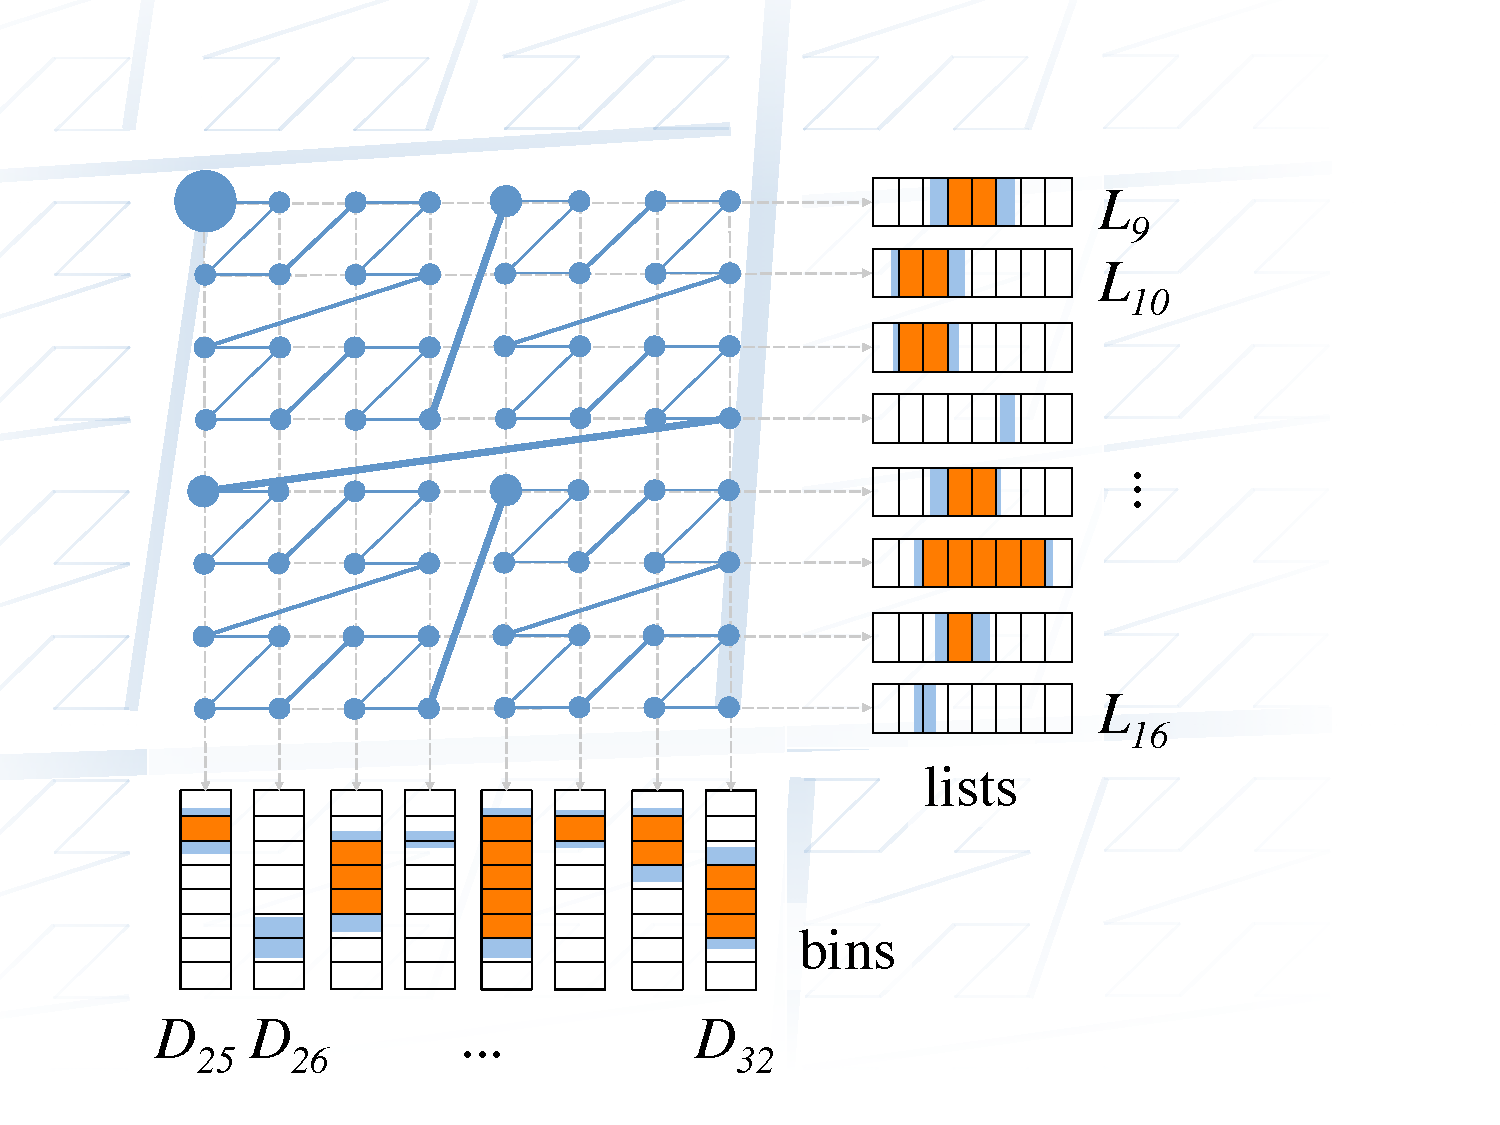
\includegraphics[scale=.35]{bin-construction.pdf}
%\end{center}
\caption{Example $2^r$ by $2^r$ (for $r=3$) region of a $Z$-order traversal of 
the bin number $\times$ list number iteration space.  During the course of the
execution of this example region there are $8$ lists and $8$ 
bins active.  The blue regions represent cache blocks which
are partially read (lists $L_9 \ldots L_{16}$) and partially written 
(bins $D_{25} \ldots D_{32}$).  The orange blocks are those which are fully read or 
written, respectively.}
\label{fig:range_coalescing} 
\end{figure}


\begin{theorem}
Given a sorted list of $O(n)$ splitters $S$ and $k$ sorted $n$-length lists 
$L_1 \ldots L_k$, the bins for a range coalescing data structure can be constructed
deterministically and cache-obliviously using $O(nk/B)$ memory transfers.
\end{theorem}

\begin{proof}
Consider a $2^r$ by $2^r$ naturally aligned region in the bin number $\times$ list
number iteration space, like the one depicted in 
\figref{range_coalescing}.\footnote{A naturally aligned region
of size $c$ by $c$ is one which begins with some indices $i \equiv 1 \pmod{c}$ 
in one dimension and $j \equiv 1 \pmod{c}$ in the other.}  
The cache need only keep the head of each of the $2^r$ constituent
lists $L_{i2^r + 1} \ldots L_{(i+1)2^r}$ for some $i$ and the head of the $2^r$ bins 
$D_{j2^r + 1} \ldots D_{(j+1)2^r}$ for some $j$. 
The ''head'' of a list is the current location
in the list as the list is streamed linearly to transfer the elements to various bins.  
For the head of each list, there can be as many as
two non-full memory tranfers (ie. not all of the elements on the cache block were
written or read).  Consider the largest $r$ for which these $2 \cdot 2^r$ list heads
fit in cache, so that $a2^r = M$ for some constant $a$.  In total, there will be 
$nk/2^{2r}$ cache flushes for a total of $M \cdot nka^2/M^2 = O(nk/B)$ cache blocks, 
assuming $M = \Omega(B)$.  There may also be additional full memory transfers in the
course of processing each $2^r$ by $2^r$ region, though
each element may appear in at most one full memory transfer, thus there are at most
$nk/B$ full memory transfers.  
\end{proof}

\subsection*{Finding splitters for small $k$}

In this section, we show how to find ''splitters'' which are representative elements
which partition all of the elements into ''bins'', each of which stores the answers to any
query which falls in the range of values between the associated splitter and the
splitter for the next bin of larger value range.
When $k$ is less than $\lg^2 n$, we can randomly select elements to be splitters
with probability $1/k$ and subdivide bins that are too large, potentially generating
extra splitters, while generating $O(N/B)$ memory transfers with high
probability, where $N=nk$.\footnote{In this context, 'with high probability' means with probability greater
than $1-1/N^c$ where $N$ is the total number of elements in the problem and $c > 1$
is some constant.} First, we establish two straightforward yet useful lemmas.

\begin{lemma}
  Consider a coin with heads probability $1/k$.  In $nk$ flips we will see
  between $n/2$ and $2n$ heads with probability at least $1-1/N^c$ for some $c>1$.
  \label{lem:number_of_flips}
\end{lemma}
\begin{proof}
  The proof follows from an application of Hoeffding's inequality, for sufficiently
  large $n$ and the assumption that $k < \lg ^2 n$.
\end{proof}

\begin{lemma}
  The largest number of elements with value between two splitters selected randomly 
  with probability $1/k$ is $(1+\epsilon)k\lg N$ with probability at least 
  $1 - 1/N^\epsilon$ for any $\epsilon > 0$.
  \label{lem:max_R}
\end{lemma}
\begin{proof}
  We can think of a bin as being created by successive coin flips with probability
  of heads equal to $1/k$: every time tails comes up, the bin grows by one.  Thus,
  the probability that a bin is of a particular size $R$ is at most $(1-1/k)^R / k$.
  Summing from $R=R'$ to $\infty$, we can bound the probability that a particular
  bin has size at least $R'$: $\sum_{R=R'}^{\infty}(1-1/k)^R/k = (1-1/k)^{R'}$.
  Letting $R'=(1+\epsilon)k\lg N$ and taking the union bound across at most $N$
  different bins, the proof follows.
\end{proof}

Consider the process of splitting a bin which exceeds $2(1+\epsilon)k$ elements.  We use 
$\floor{R/2(1+\epsilon)k}$ applications of a cache-oblivious selection 
algorithm~\cite{FrigoLePr99} to subdivide large bins of size $R$ into bins of 
size at most $2(1+\epsilon)k$ elements using $O(\floor{R/2(1+\epsilon)k} R/B)$ 
memory transfers.\footnote{For
convenience, we assume $R>B$.  There is no need to make the bins smaller than $B$
elements, since processing a bin incurs at least one memory reference.}

\begin{theorem}
  Let $N=nk$.  The total number of memory transfers $S$ required to subdivide all $m$ bins to be less
  than $2(1+\epsilon)k$ elements each is $O(N/B)$, assuming that the largest bin is at most 
  $(1+\epsilon)k\lg N$ elements and $n/2 \leq m \leq 2n$.
\end{theorem}
\begin{proof}
  Let $x_i$ be the number of memory transfers incurred by the $i$th bin and
  thus $S=\sum_{i=1}^{m}X_i$.  Then, we have 
  \begin{align*}
    E[x_i] & \leq a \sum_{R=0}^{\infty} \frac{1}{k}\paren{1-\frac{1}{k}}^R \floor{\frac{R}{2(1+\epsilon)k}} \frac{R}{B}\\
    & \leq a \sum_{R=0}^{\infty} \paren{1-\frac{1}{k}}^R \frac{R^2}{2(1+\epsilon)k^2B}\\
    & \leq a\frac{k}{B}\\
  \end{align*}
  for some constant $a>0$.
  Also, we see that
  \begin{align*}
    x_i &\leq \floor{\frac{(1+\epsilon)k\lg N}{2(1+\epsilon)k}}\frac{(1+\epsilon)k\lg N}{B}\\
    &\leq \frac{k}{2B}(1+\epsilon) \lg ^2 N \\
  \end{align*}
  for all $i$.  Let $t = \paren{k/2B}(1+\epsilon) \lg ^2 N$.  
  Thus each random variable in $\{ x_1 \ldots x_m \}$ has support
  in the range $[0, t]$.
  A Hoeffding bound on $S$ gives us
  \begin{align*}
    %\prob{S - E[S] \geq E[S]} & \leq \exp \paren{ -\frac{2\paren{ am\frac{k}{B}}^2}{m\paren{\frac{k}{2B}\paren{1+\epsilon}^2\lg^2 N}^2}}\\
    \prob{S - E[S] \geq t \sqrt{\epsilon m \lg N}} & \leq \exp \paren{-2\frac{\epsilon \lg N m t^2}{mt^2}}\\
    & \leq \exp \paren{-2\epsilon \lg N}\\
    & \leq N^{-\epsilon}.\\
  \end{align*}
  For sufficiently large $N$, $S$ is $O(N/B)$ with high probability.
\end{proof}

We need to verify that the process of subdivision does not unduly increase the number
of bins.

\begin{lemma}
After subdivision, we will have $O(n)$ bins.
\end{lemma}
\begin{proof}
Initially, there are $O(n)$ splitters with high probability by \lemref{number_of_flips}.
The process of subdividing bins generates bins with size at least $k$, thus we
can create at most $N/k = n$ extra bins through subdivision.
\end{proof}

\subsection*{Finding splitters for large $k$}

When $k$ is at least $\lg ^2 n$, we use an oversampling technique as used in 
sample sort~\cite{BlellochLeMa91} to find a set of splitters and bound the 
size of all bins.  In particular, we start by randomly sampling elements as 
candidate splitters with probability $1/\lg k$.  Then, we merge these candidates
using and a cache-oblivious $k$-merger~\cite{FrigoLePr99} using 
$O((N/B\lg k) \log_{M/B} (k/B) + k) = O(N/B)$ memory transfers.  Finally, we take
every $n$ evenly space elements from this sorted list as our set of splitters.

\begin{theorem}
  Given an oversampling rate of $k/\lg k$, the largest resulting bin has at least 
  $2(1+\epsilon)k$ elements with probability less than $N^{-\epsilon}$.
\end{theorem}
\begin{proof}
  Let $R$ be the size of the largest bin.  
  From Theorem B.3 of~\cite{BlellochLeMa91} and sufficiently large $N$, 
  we have that $\prob{R > 2(1+\epsilon)k}$
  \begin{align*}
    &\leq N \exp \paren{ -(1+\epsilon)\paren{\frac{1+2\epsilon}{2(1+\epsilon)}}^2 \frac{k}{\lg k} }\\
    &\leq N \exp \paren{-(1+\epsilon)\frac{k}{4\lg k}}\\
    &\leq N \exp \paren{-(1+\epsilon)\frac{\lg^2 \frac{N}{\lg^2 n}}{4 \lg \lg ^2 n}}\\
    &\leq N \exp \paren{-(1+\epsilon)\frac{\lg^2 N - 4 \lg N \lg \lg n + 4\lg ^2 \lg n }{8 \lg \lg n}}\\
    &\leq N \exp \paren{-(1+\epsilon)\lg N}\\
    &\leq N^{-\epsilon}\\
  \end{align*}
\end{proof}



